\documentclass[11pt,a4paper,english]{article}
\usepackage[T1]{fontenc}
\usepackage[utf8]{inputenc}
\usepackage{babel}
\usepackage{blindtext}
\usepackage{hyperref}
\usepackage{graphicx}

\setlength\fboxsep{0.25cm}
\setlength\fboxrule{0pt}


\title{Correlation of Forum Activity and real world events based on a social network dataset}
\author{%
  Cedric Waldburger\thanks{data provided by ASmallWorld Ltd, New York}\\
  \small Department of Electrical Engineering\\
  \small ETH Zurich \\
  \small\texttt{ctwaldburger@student.ust.hk}
  \and
  Christoffer Hirsimaa\\
  \small Department of Computer Science\\
  \small KTH Stockholm\\
  \small\texttt{cahirsimaa@stu.ust.hk}
}

\begin{document}
  \maketitle

  \begin{abstract}
    We've used the data from invitation-only network ASmallWorld.net to analyze correlations of forum activity and real life events.
  \end{abstract}
  \newpage

  \tableofcontents\newpage

	\section{The Data}
		\subsection{About ASmallWorld}
			ASmallWorld.net is a unique social media combining a by-invitation-only social network with a content delivery platform targeting the "upper end" of the social media market. We are the market leader in our segment. As An integrated media company, ASW is an ideal match for advertisers seeking to target the world$\prime$s tastemakers and develop heightened mindshare with this sophisticated and influential group.
			
		\subsection{Facts \& Figures}
			\begin{itemize}
				\item \bf Total number of records: \rm 254 622
				\item \bf First record: \rm June 7, 2004
				\item \bf Last record: \rm February 2, 2011
			\end{itemize}
 \newpage
 		
	\section{Visualization}
	
	\section{Experiments - News Events}
			\subsection{2005}
			\href{http://politicom.moldova.org/news/10-most-important-world-events-of-2005-7712-eng.html}{Top10 Events in 2005 on moldova.org}
				\begin{itemize}
				\item \bf Death of Pope John Paul II\rm
					\\ The death of Pope John Paul II marked the end of an era in the life of the Roman-Catholic Church and modern history. 
					\\\\ \bf time span: \rm April 2 - April 9
					\\ \bf geographical area: \rm Vatican
					\\ \bf total number of threads: \rm 0
					
					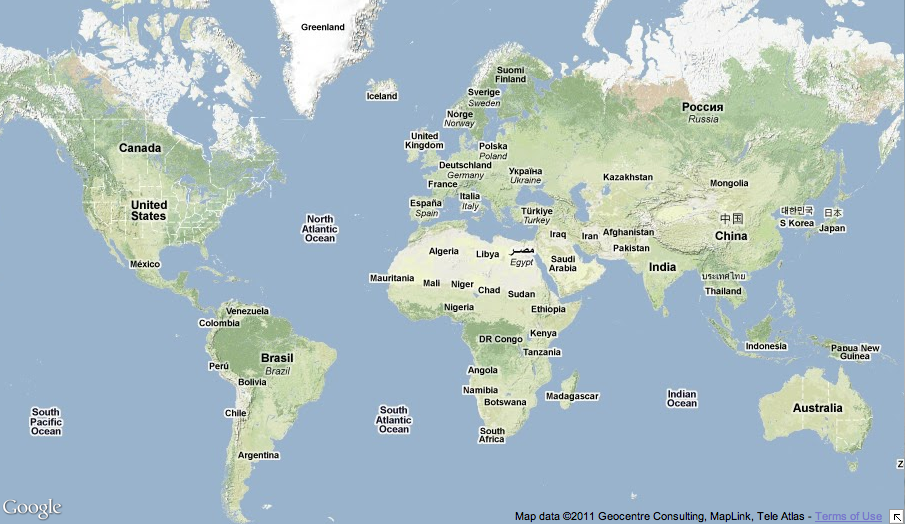
\includegraphics[width=130mm]{img/2005-1}
						
					\bf interpretation: \rm YES OR NO - ARE WE IMPRESSED? :)
						


				\item \bf Terrorist act in London \rm
					\\ A terrorist act in London overshadowed the G8 summit in Gleneagles, Scotland, and spoiled Britons' joy over London's election as the host city for the 2012 Olympics. Four explosive devices went off in the underground and a bus, leaving 50 people dead and about 700 injured.
					\\\\ \bf time span: \rm July 7 - July 21
					\\ \bf geographical area: \rm London, UK
					\\ \bf total number of threads: \rm 0
					
					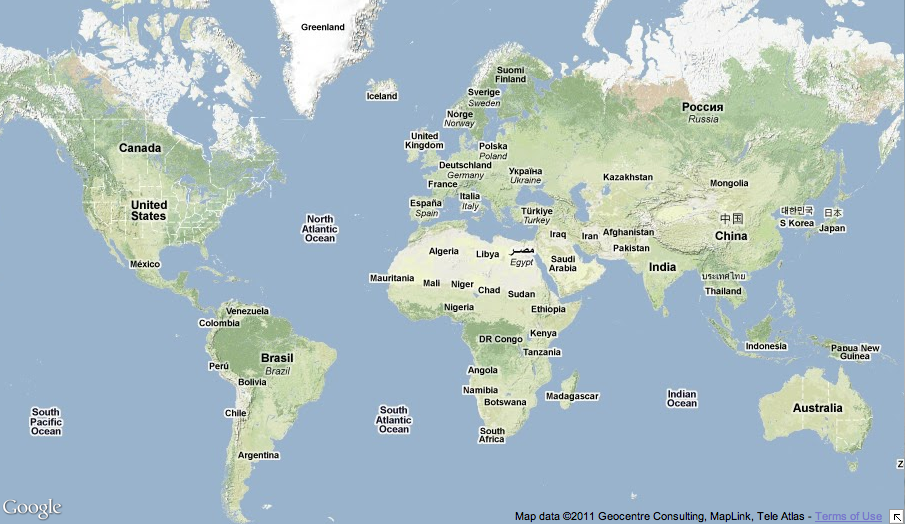
\includegraphics[width=130mm]{img/2005-1}
					
					\bf interpretation: \rm YES OR NO - ARE WE IMPRESSED? :)


						
				\item \bf Hurricane Katrina \rm
					\\ Hurricane Katrina in the United States showed that the world's leading super power was unprepared to deal with the aftermath of the natural disaster. The hurricane destroyed the cradle of jazz, New Orleans. 
					\\\\ \bf time span: \rm August 23 - September 23
					\\ \bf geographical area: \rm New Orleans, USA
					\\ \bf total number of threads: \rm 0
					
					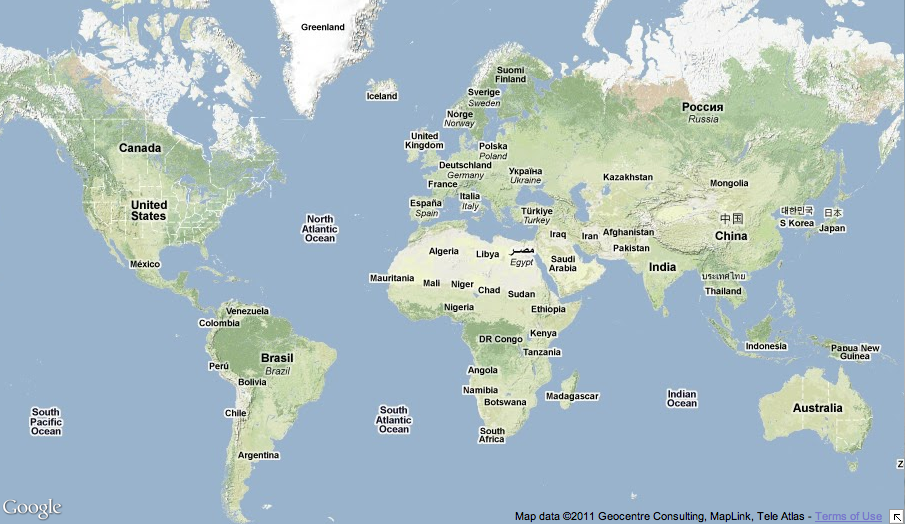
\includegraphics[width=130mm]{img/2005-1}
					
					\bf interpretation: \rm YES OR NO - ARE WE IMPRESSED? :)
					
					
												
				\end{itemize}
			
			\subsection{2006}
			\href{http://social.moldova.org/news/10-most-important-world-events-of-2006-217385-eng.html}{Top10 Events in 2006 on moldova.org}
				\begin{itemize}
					\item \bf Bird Flu \rm
						\\ People watched nervously as the infamous disease spread from Asia to Europe. But flu season died down before disaster struck. The human being was in a big danger, as a current H5N1 strain is a fast-mutating, highly pathogenic avian influenza virus (HPAI) found in multiple bird species.
						\\\\ \bf time span: \rm January 1 - January 14
						\\ \bf geographical area: \rm Asia
						\\ \bf total number of threads: \rm 0
						
						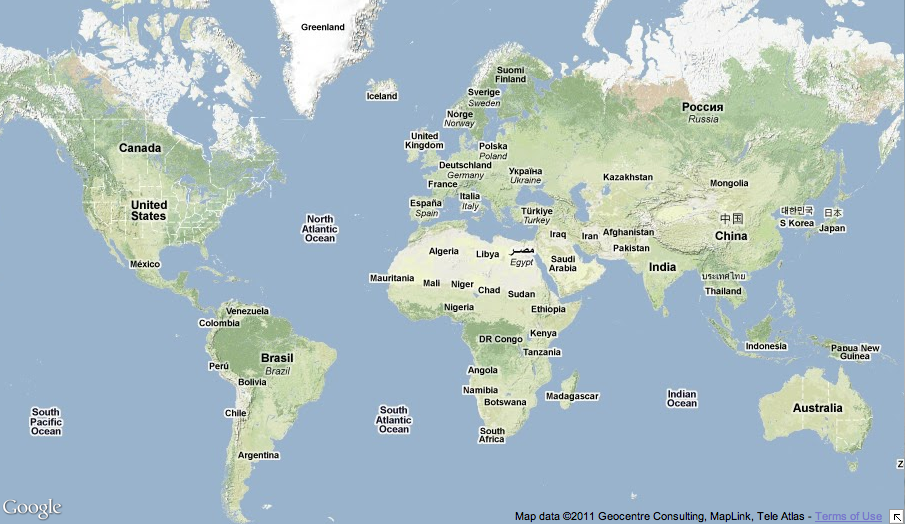
\includegraphics[width=130mm]{img/2005-1}
						
						\bf interpretation: \rm YES OR NO - ARE WE IMPRESSED? :)
					
					
					
					\item \bf Soccer World Cup \rm
						\\ Italy wins the World Cup 5-3 vs. France.
						\\\\ \bf time span: \rm June 9 - July 9
						\\ \bf geographical area: \rm Germany, Italy
						\\ \bf total number of threads: \rm 0
						
						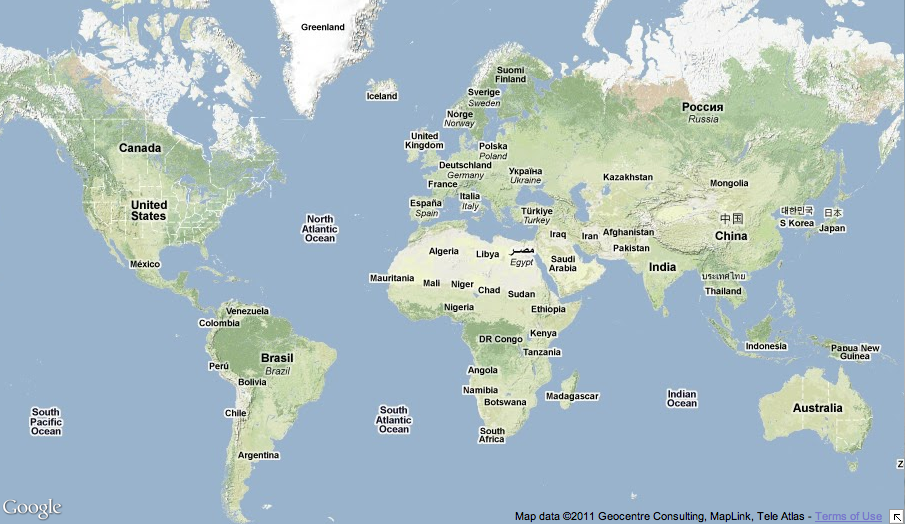
\includegraphics[width=130mm]{img/2005-1}
						
						\bf interpretation: \rm YES OR NO - ARE WE IMPRESSED? :)
						
						
					
					\item \bf Saddam Hussein sentenced to death \rm
						\\ Saddam Hussein sentenced to death by hanging by an Iraqi court. Earlier in this year he was charged with genocide by an Iraqi court for a campaign against Iraq's Kurdish population in 1988.
					\\\\ \bf time span: \rm November 5 - November 12
					\\ \bf geographical area: \rm Iraq
					\\ \bf total number of threads: \rm 0
						
					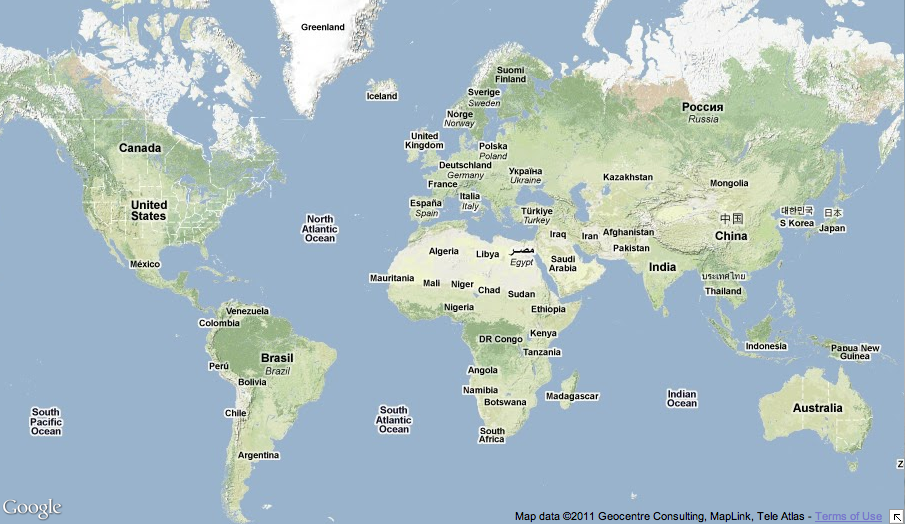
\includegraphics[width=130mm]{img/2005-1}
						
					\bf interpretation: \rm YES OR NO - ARE WE IMPRESSED? :)
						
						
							
				\end{itemize}
			
			\subsection{2007}
			\href{http://social.moldova.org/news/10-most-important-world-events-of-2007-217388-eng.html}{Top10 Events in 2007 on moldova.org}
				\begin{itemize}
					\item \bf Gordon Brown becomes Prime Minister \rm
						\\ Gordon Brown replaces Tony Blair as the prime minister of Great Britain (June 27). "Let the work of change begin," said Brown in the day he was elected.
						\\\\ \bf time span: \rm June 27 - July 4
						\\ \bf geographical area: \rm UK
						\\ \bf total number of threads: \rm 0
					
						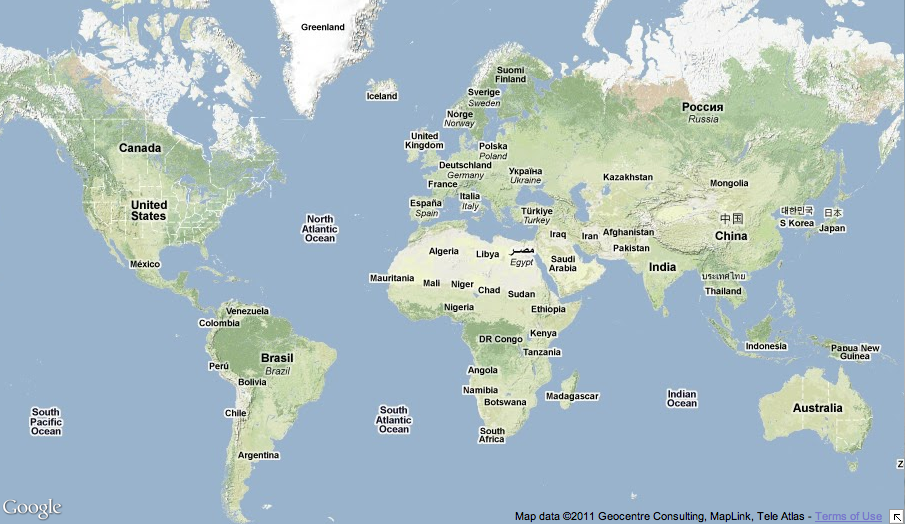
\includegraphics[width=130mm]{img/2005-1}
						
						\bf interpretation: \rm YES OR NO - ARE WE IMPRESSED? :)
						
						
						
					\item \bf Chile Earthquake \rm
						\\ 8.0 Earthquake in Peru kills over 500 people, injures over 1,500; 7.7 Earthquake in northern Chile.
						\\\\ \bf time span: \rm August 15 - August 29
						\\ \bf geographical area: \rm South America
						\\ \bf total number of threads: \rm 0
					
						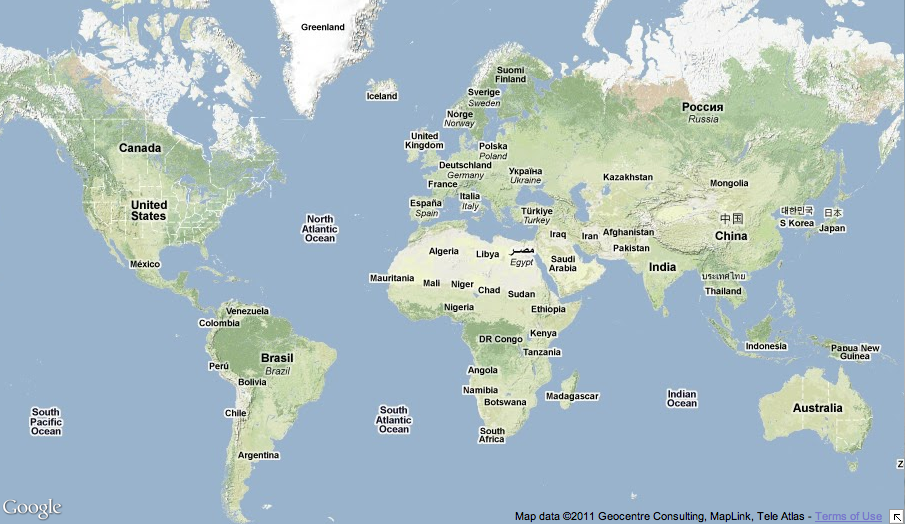
\includegraphics[width=130mm]{img/2005-1}
						
						\bf interpretation: \rm YES OR NO - ARE WE IMPRESSED? :)
						
						
						
					\item \bf Writers Guild goes on strike \rm
						\\ The Writers Guild of America goes on a strike that lasts until February 12, 2008. More than 12,000 writers joined the strike. The strike's goal was to rectify what was perceived as a historical injustice to America: the greatly diminished monetary compensation the writers got in comparison with the profits of the larger studios. The guilds were on strike 100 days.
						\\\\ \bf time span: \rm November - December
						\\ \bf geographical area: \rm Los Angeles, USA
						\\ \bf total number of threads: \rm 0
					
						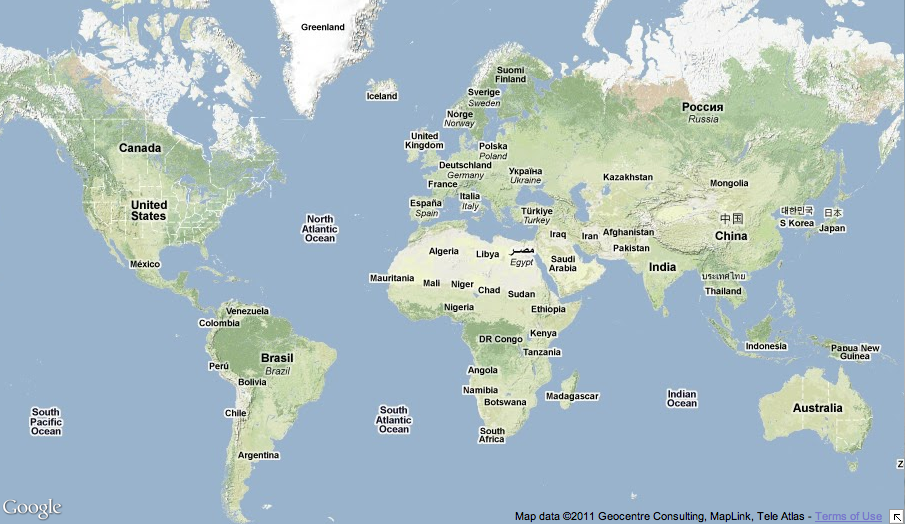
\includegraphics[width=130mm]{img/2005-1}
						
						\bf interpretation: \rm YES OR NO - ARE WE IMPRESSED? :)
						
						
						
				\end{itemize}
			
			\subsection{2008}
			\href{http://social.moldova.org/news/10-most-important-world-events-of-2008-217389-eng.html}{Top10 Events in 2008 on moldova.org}
				\begin{itemize}
					\item \bf Kosovo declares independency \rm
						\\ Kosovo declares independence from Serbia, announced by prime minister Hashim Thaci. Serbian prime minister Vojislav Kostunica says he would never recognize the "false state." International reaction is mixed, with the United States, France, Germany, and Britain indicating that they plan to recognize Kosovo as the world's 195th country.
						\\\\ \bf time span: \rm February 17 - March 17
						\\ \bf geographical area: \rm Kosovo
						\\ \bf total number of threads: \rm 0
					
						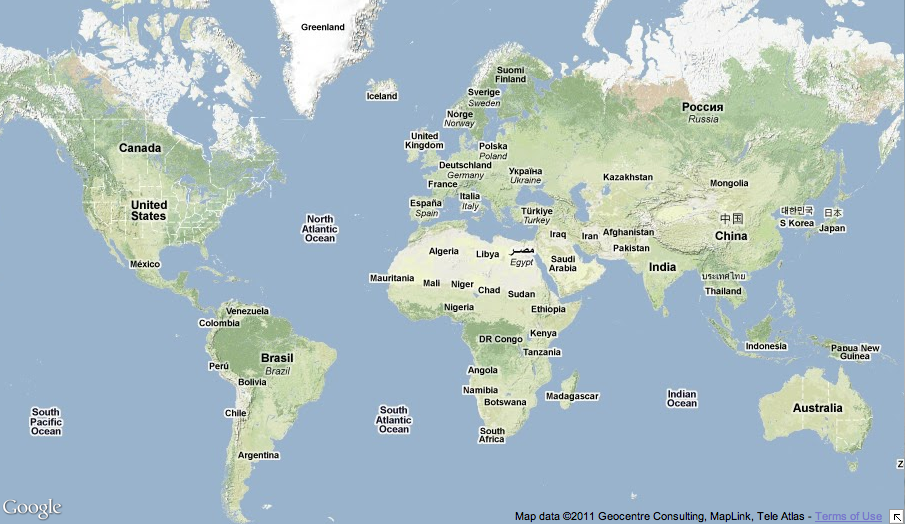
\includegraphics[width=130mm]{img/2005-1}
						
						\bf interpretation: \rm YES OR NO - ARE WE IMPRESSED? :)
						
						
						
					\item \bf Medvedev becomes Russia's President \rm
						\\ Russia in 2008 chooses another president - Dmitri A. Medvedev, a former aide to Russian president Vladimir Putin, wins the presidential election in a landslide. Putin will remain in a position of power, serving as Medvedev's prime minister.
						\\\\ \bf time span: \rm March 2 - March 9
						\\ \bf geographical area: \rm Russia
						\\ \bf total number of threads: \rm 0
						
						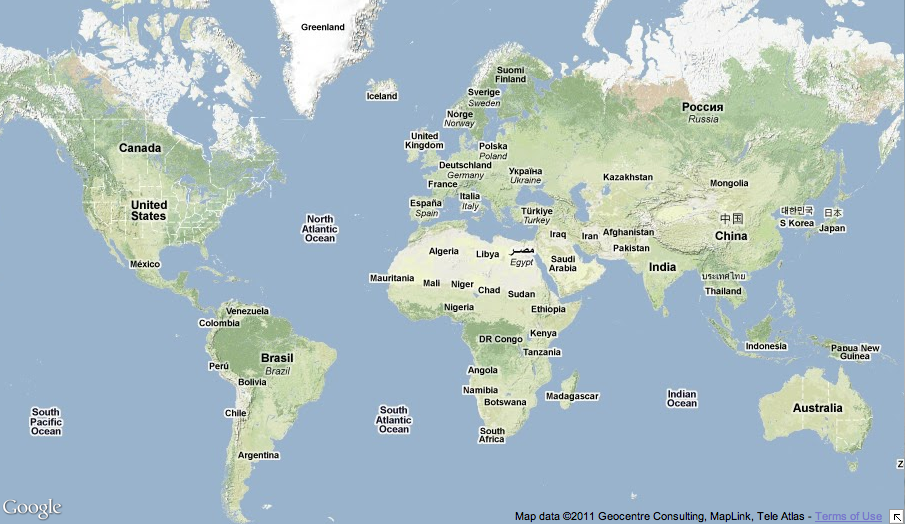
\includegraphics[width=130mm]{img/2005-1}
						
						\bf interpretation: \rm YES OR NO - ARE WE IMPRESSED? :)
					
					
					\item \bf China's Earthquake \rm
						\\On May 12, 2008, a magnitude 7.9 earthquake struck the Sichuan Province of China, killing more than 69,000 people, making it China's worst disaster in more than 30 years.
						\\\\ \bf time span: \rm May 12 - May 28
						\\ \bf geographical area: \rm China
						\\ \bf total number of threads: \rm 0
						
						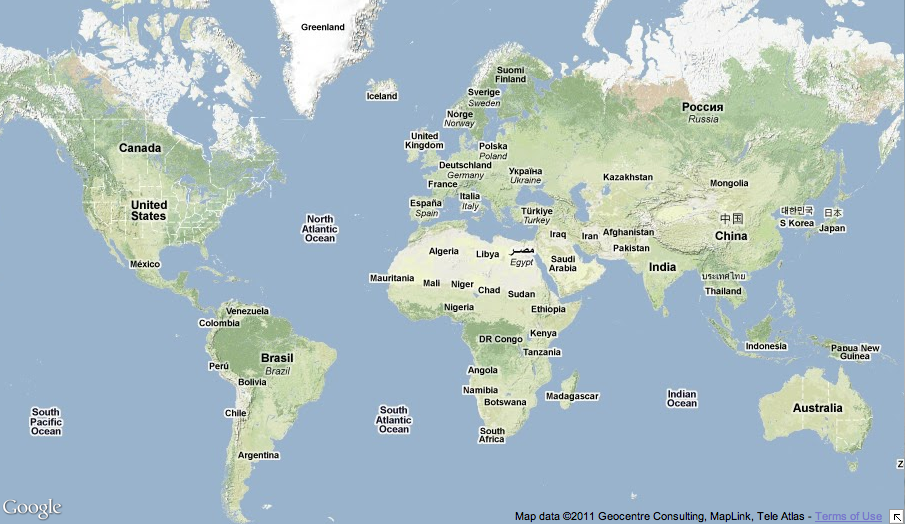
\includegraphics[width=130mm]{img/2005-1}
						\bf interpretation: \rm YES OR NO - ARE WE IMPRESSED? :)
						
						
					
						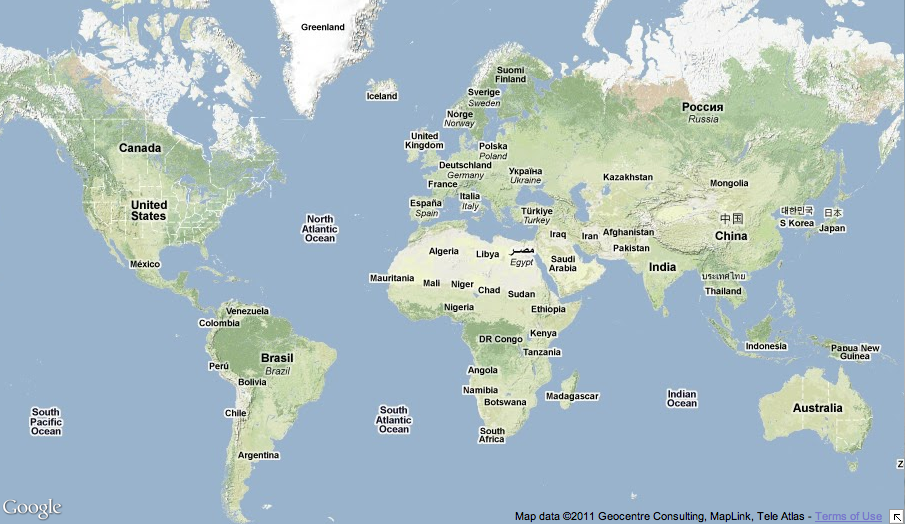
\includegraphics[width=130mm]{img/2005-1}
						
						\bf interpretation: \rm YES OR NO - ARE WE IMPRESSED? :)
						
						

					\item \bf Summer Olympic Games \rm
						\\ Summer Olympic Games 2008 that took place in Beijing, China. It was the XXIX Olympiad. The international multi-sport event officially opened on August 6 and ended on August 24, featuring 10,500 athletes who struggled for the Olympic Gold medal in 302 events in 28 sports. The Summer Olympic Games 2008 was really worth remembering, showing remarkable performances of the athletes: 43 new world records and 132 new Olympic records. Besides, representative of 87 countries won at least one medal at these Olympics, an unprecedented achievement.
						\\\\ \bf time span: \rm August 8 - 24
						\\ \bf geographical area: \rm Beijing, China
						\\ \bf total number of threads: \rm 0
					
						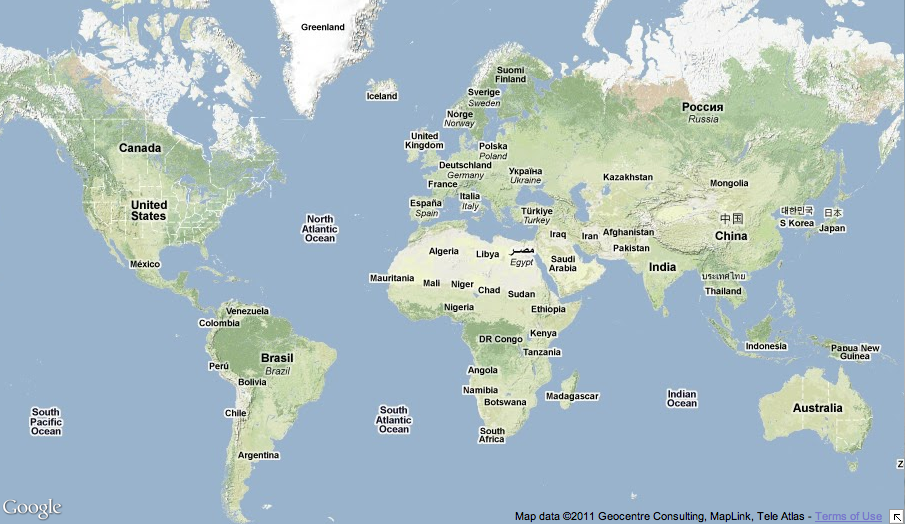
\includegraphics[width=130mm]{img/2005-1}
						
						\bf interpretation: \rm YES OR NO - ARE WE IMPRESSED? :)
						
						
						
				\end{itemize}
			
			\subsection{2009}
			\href{http://social.moldova.org/news/10-most-important-world-events-of-2009-217390-eng.html}{Top10 Events in 2009 on moldova.org}
				\begin{itemize}
					\item \bf Swine Flu \rm
						\\ The "swine flu", the H1N1 influenza strain is the first condition deemed a global pandemic since the Hong Kong flu of 1967 to 1968. According to the latest WHO statistics, the virus has killed more than 18,000 people since it appeared in April 2009 and were 622,482 infected (approximate).
						\\\\ \bf time span: \rm --
						\\ \bf geographical area: \rm --
						\\ \bf total number of threads: \rm 0
						
						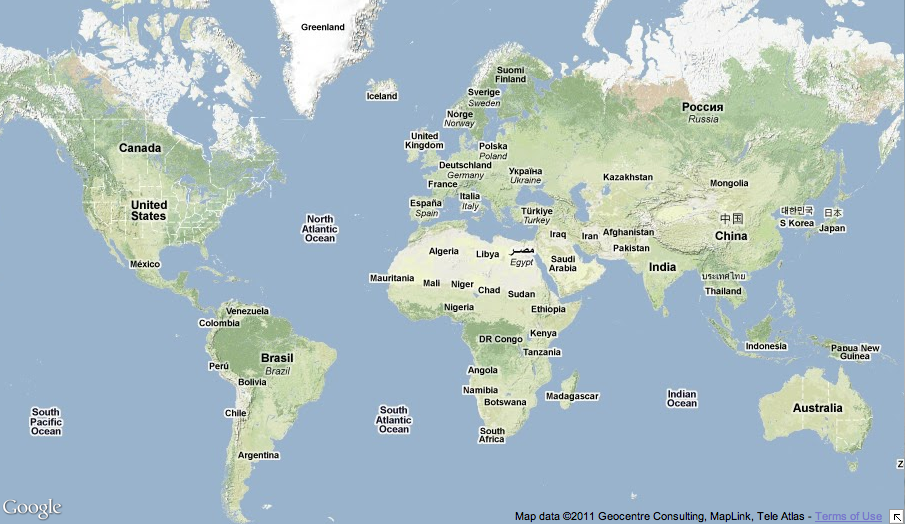
\includegraphics[width=130mm]{img/2005-1}
						
						\bf interpretation: \rm YES OR NO - ARE WE IMPRESSED? :)
						
						
						
					\item \bf Michael Jackson's death \rm
						\\ Michael Jackson the most famous US singer dies after he suffered cardiac arrest at his home in the Holmby Hills neighborhood in Los Angeles, California. Later the Los Angeles County Coroner declared Jackson's death a homicide caused by the combination of drugs in his body.
\\ Conrad Murray is the doctor that had to take care of Michael$\prime$ s health before his death, and in 2011 he is still under charge of involuntary manslaughter. Internet traffic reaches unprecedented levels after entertainer Michael Jackson's death triggers an outpouring of worldwide grief.
						\\\\ \bf time span: \rm June 25 - July 2
						\\ \bf geographical area: \rm USA
						\\ \bf total number of threads: \rm 0
						
						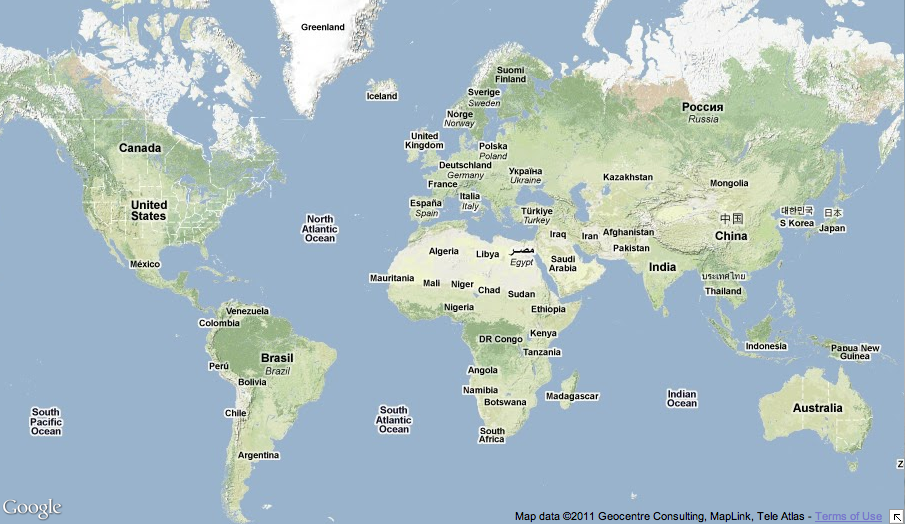
\includegraphics[width=130mm]{img/2005-1}
						
						\bf interpretation: \rm YES OR NO - ARE WE IMPRESSED? :)
						
						
						
					\item \bf Silvio Berlusconi attacked \rm
						\\ Italian Prime Minister Silvio Burlusconi is knocked to the ground and hit in the face after a political rally in Milan, Italy. An attacker hurled a statuette at Italian Premier striking the leader in the face. The attacker is a 42-year-old Massimo Tartaglia, a graphic designer with a history of mental problems. The attack occurred at a difficult political time for Berlusconi, who has been plagued by scandals.
						\\\\ \bf time span: \rm December 14 - December 28
						\\ \bf geographical area: \rm Italy
						\\ \bf total number of threads: \rm 0
						
						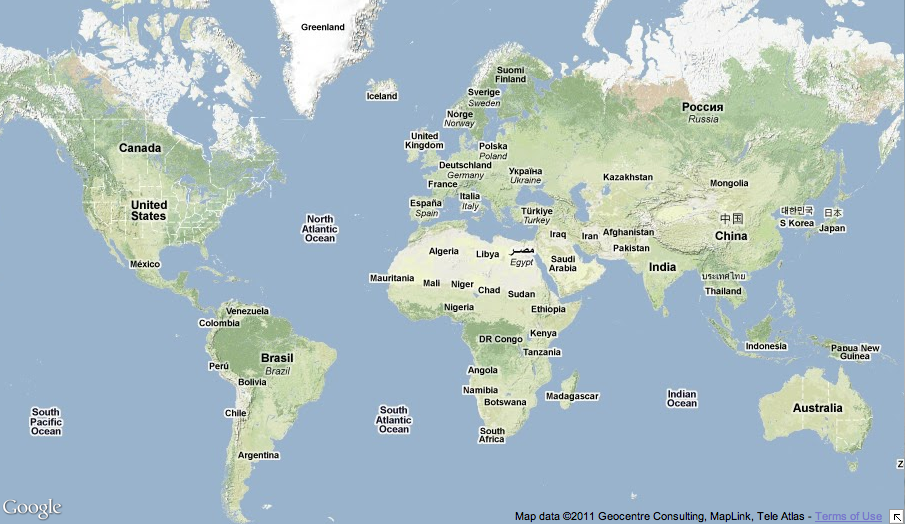
\includegraphics[width=130mm]{img/2005-1}
						
						\bf interpretation: \rm YES OR NO - ARE WE IMPRESSED? :)
						
					
						
				\end{itemize}
 \newpage	
	\section{Conclusion}

\end{document}